\documentclass[xcolor=x11names,compress]{beamer}

%% General document %%%%%%%%%%%%%%%%%%%%%%%%%%%%%%%%%%
\usepackage{graphicx}
\graphicspath{{graphics/}}
\usepackage{animate}
\usepackage{tikz}

% ########For highlight boxes over equations########
\usepackage{color}
\definecolor{AliceBlue}{rgb}{0.94,0.97,1.00}
\definecolor{AntiqueWhite1}{rgb}{1.00,0.94,0.86}
\definecolor{AntiqueWhite2}{rgb}{0.93,0.87,0.80}
\definecolor{AntiqueWhite3}{rgb}{0.80,0.75,0.69}
\definecolor{AntiqueWhite4}{rgb}{0.55,0.51,0.47}
\definecolor{AntiqueWhite}{rgb}{0.98,0.92,0.84}
\definecolor{BlanchedAlmond}{rgb}{1.00,0.92,0.80}
\definecolor{BlueViolet}{rgb}{0.54,0.17,0.89}
\definecolor{CadetBlue1}{rgb}{0.60,0.96,1.00}
\definecolor{CadetBlue2}{rgb}{0.56,0.90,0.93}
\definecolor{CadetBlue3}{rgb}{0.48,0.77,0.80}
\definecolor{CadetBlue4}{rgb}{0.33,0.53,0.55}
\definecolor{CadetBlue}{rgb}{0.37,0.62,0.63}
\definecolor{CornflowerBlue}{rgb}{0.39,0.58,0.93}
\definecolor{DarkBlue}{rgb}{0.00,0.00,0.55}
\definecolor{DarkCyan}{rgb}{0.00,0.55,0.55}
\definecolor{DarkGoldenrod1}{rgb}{1.00,0.73,0.06}
\definecolor{DarkGoldenrod2}{rgb}{0.93,0.68,0.05}
\definecolor{DarkGoldenrod3}{rgb}{0.80,0.58,0.05}
\definecolor{DarkGoldenrod4}{rgb}{0.55,0.40,0.03}
\definecolor{DarkGoldenrod}{rgb}{0.72,0.53,0.04}
\definecolor{DarkGray}{rgb}{0.66,0.66,0.66}
\definecolor{DarkGreen}{rgb}{0.00,0.39,0.00}
\definecolor{DarkGrey}{rgb}{0.66,0.66,0.66}
\definecolor{DarkKhaki}{rgb}{0.74,0.72,0.42}
\definecolor{DarkMagenta}{rgb}{0.55,0.00,0.55}
\definecolor{DarkOliveGreen1}{rgb}{0.79,1.00,0.44}
\definecolor{DarkOliveGreen2}{rgb}{0.74,0.93,0.41}
\definecolor{DarkOliveGreen3}{rgb}{0.64,0.80,0.35}
\definecolor{DarkOliveGreen4}{rgb}{0.43,0.55,0.24}
\definecolor{DarkOliveGreen}{rgb}{0.33,0.42,0.18}
\definecolor{DarkOrange1}{rgb}{1.00,0.50,0.00}
\definecolor{DarkOrange2}{rgb}{0.93,0.46,0.00}
\definecolor{DarkOrange3}{rgb}{0.80,0.40,0.00}
\definecolor{DarkOrange4}{rgb}{0.55,0.27,0.00}
\definecolor{DarkOrange}{rgb}{1.00,0.55,0.00}
\definecolor{DarkOrchid1}{rgb}{0.75,0.24,1.00}
\definecolor{DarkOrchid2}{rgb}{0.70,0.23,0.93}
\definecolor{DarkOrchid3}{rgb}{0.60,0.20,0.80}
\definecolor{DarkOrchid4}{rgb}{0.41,0.13,0.55}
\definecolor{DarkOrchid}{rgb}{0.60,0.20,0.80}
\definecolor{DarkRed}{rgb}{0.55,0.00,0.00}
\definecolor{DarkSalmon}{rgb}{0.91,0.59,0.48}
\definecolor{DarkSeaGreen1}{rgb}{0.76,1.00,0.76}
\definecolor{DarkSeaGreen2}{rgb}{0.71,0.93,0.71}
\definecolor{DarkSeaGreen3}{rgb}{0.61,0.80,0.61}
\definecolor{DarkSeaGreen4}{rgb}{0.41,0.55,0.41}
\definecolor{DarkSeaGreen}{rgb}{0.56,0.74,0.56}
\definecolor{DarkSlateBlue}{rgb}{0.28,0.24,0.55}
\definecolor{DarkSlateGray1}{rgb}{0.59,1.00,1.00}
\definecolor{DarkSlateGray2}{rgb}{0.55,0.93,0.93}
\definecolor{DarkSlateGray3}{rgb}{0.47,0.80,0.80}
\definecolor{DarkSlateGray4}{rgb}{0.32,0.55,0.55}
\definecolor{DarkSlateGray}{rgb}{0.18,0.31,0.31}
\definecolor{DarkSlateGrey}{rgb}{0.18,0.31,0.31}
\definecolor{DarkTurquoise}{rgb}{0.00,0.81,0.82}
\definecolor{DarkViolet}{rgb}{0.58,0.00,0.83}
\definecolor{DeepPink1}{rgb}{1.00,0.08,0.58}
\definecolor{DeepPink2}{rgb}{0.93,0.07,0.54}
\definecolor{DeepPink3}{rgb}{0.80,0.06,0.46}
\definecolor{DeepPink4}{rgb}{0.55,0.04,0.31}
\definecolor{DeepPink}{rgb}{1.00,0.08,0.58}
\definecolor{DeepSkyBlue1}{rgb}{0.00,0.75,1.00}
\definecolor{DeepSkyBlue2}{rgb}{0.00,0.70,0.93}
\definecolor{DeepSkyBlue3}{rgb}{0.00,0.60,0.80}
\definecolor{DeepSkyBlue4}{rgb}{0.00,0.41,0.55}
\definecolor{DeepSkyBlue}{rgb}{0.00,0.75,1.00}
\definecolor{DimGray}{rgb}{0.41,0.41,0.41}
\definecolor{DimGrey}{rgb}{0.41,0.41,0.41}
\definecolor{DodgerBlue1}{rgb}{0.12,0.56,1.00}
\definecolor{DodgerBlue2}{rgb}{0.11,0.53,0.93}
\definecolor{DodgerBlue3}{rgb}{0.09,0.45,0.80}
\definecolor{DodgerBlue4}{rgb}{0.06,0.31,0.55}
\definecolor{DodgerBlue}{rgb}{0.12,0.56,1.00}
\definecolor{FloralWhite}{rgb}{1.00,0.98,0.94}
\definecolor{ForestGreen}{rgb}{0.13,0.55,0.13}
\definecolor{GhostWhite}{rgb}{0.97,0.97,1.00}
\definecolor{GreenYellow}{rgb}{0.68,1.00,0.18}
\definecolor{HotPink1}{rgb}{1.00,0.43,0.71}
\definecolor{HotPink2}{rgb}{0.93,0.42,0.65}
\definecolor{HotPink3}{rgb}{0.80,0.38,0.56}
\definecolor{HotPink4}{rgb}{0.55,0.23,0.38}
\definecolor{HotPink}{rgb}{1.00,0.41,0.71}
\definecolor{IndianRed1}{rgb}{1.00,0.42,0.42}
\definecolor{IndianRed2}{rgb}{0.93,0.39,0.39}
\definecolor{IndianRed3}{rgb}{0.80,0.33,0.33}
\definecolor{IndianRed4}{rgb}{0.55,0.23,0.23}
\definecolor{IndianRed}{rgb}{0.80,0.36,0.36}
\definecolor{LavenderBlush1}{rgb}{1.00,0.94,0.96}
\definecolor{LavenderBlush2}{rgb}{0.93,0.88,0.90}
\definecolor{LavenderBlush3}{rgb}{0.80,0.76,0.77}
\definecolor{LavenderBlush4}{rgb}{0.55,0.51,0.53}
\definecolor{LavenderBlush}{rgb}{1.00,0.94,0.96}
\definecolor{LawnGreen}{rgb}{0.49,0.99,0.00}
\definecolor{LemonChiffon1}{rgb}{1.00,0.98,0.80}
\definecolor{LemonChiffon2}{rgb}{0.93,0.91,0.75}
\definecolor{LemonChiffon3}{rgb}{0.80,0.79,0.65}
\definecolor{LemonChiffon4}{rgb}{0.55,0.54,0.44}
\definecolor{LemonChiffon}{rgb}{1.00,0.98,0.80}
\definecolor{LightBlue1}{rgb}{0.75,0.94,1.00}
\definecolor{LightBlue2}{rgb}{0.70,0.87,0.93}
\definecolor{LightBlue3}{rgb}{0.60,0.75,0.80}
\definecolor{LightBlue4}{rgb}{0.41,0.51,0.55}
\definecolor{LightBlue}{rgb}{0.68,0.85,0.90}
\definecolor{LightCoral}{rgb}{0.94,0.50,0.50}
\definecolor{LightCyan1}{rgb}{0.88,1.00,1.00}
\definecolor{LightCyan2}{rgb}{0.82,0.93,0.93}
\definecolor{LightCyan3}{rgb}{0.71,0.80,0.80}
\definecolor{LightCyan4}{rgb}{0.48,0.55,0.55}
\definecolor{LightCyan}{rgb}{0.88,1.00,1.00}
\definecolor{LightGoldenrod1}{rgb}{1.00,0.93,0.55}
\definecolor{LightGoldenrod2}{rgb}{0.93,0.86,0.51}
\definecolor{LightGoldenrod3}{rgb}{0.80,0.75,0.44}
\definecolor{LightGoldenrod4}{rgb}{0.55,0.51,0.30}
\definecolor{LightGoldenrodYellow}{rgb}{0.98,0.98,0.82}
\definecolor{LightGoldenrod}{rgb}{0.93,0.87,0.51}
\definecolor{LightGray}{rgb}{0.83,0.83,0.83}
\definecolor{LightGreen}{rgb}{0.56,0.93,0.56}
\definecolor{LightGrey}{rgb}{0.83,0.83,0.83}
\definecolor{LightPink1}{rgb}{1.00,0.68,0.73}
\definecolor{LightPink2}{rgb}{0.93,0.64,0.68}
\definecolor{LightPink3}{rgb}{0.80,0.55,0.58}
\definecolor{LightPink4}{rgb}{0.55,0.37,0.40}
\definecolor{LightPink}{rgb}{1.00,0.71,0.76}
\definecolor{LightSalmon1}{rgb}{1.00,0.63,0.48}
\definecolor{LightSalmon2}{rgb}{0.93,0.58,0.45}
\definecolor{LightSalmon3}{rgb}{0.80,0.51,0.38}
\definecolor{LightSalmon4}{rgb}{0.55,0.34,0.26}
\definecolor{LightSalmon}{rgb}{1.00,0.63,0.48}
\definecolor{LightSeaGreen}{rgb}{0.13,0.70,0.67}
\definecolor{LightSkyBlue1}{rgb}{0.69,0.89,1.00}
\definecolor{LightSkyBlue2}{rgb}{0.64,0.83,0.93}
\definecolor{LightSkyBlue3}{rgb}{0.55,0.71,0.80}
\definecolor{LightSkyBlue4}{rgb}{0.38,0.48,0.55}
\definecolor{LightSkyBlue}{rgb}{0.53,0.81,0.98}
\definecolor{LightSlateBlue}{rgb}{0.52,0.44,1.00}
\definecolor{LightSlateGray}{rgb}{0.47,0.53,0.60}
\definecolor{LightSlateGrey}{rgb}{0.47,0.53,0.60}
\definecolor{LightSteelBlue1}{rgb}{0.79,0.88,1.00}
\definecolor{LightSteelBlue2}{rgb}{0.74,0.82,0.93}
\definecolor{LightSteelBlue3}{rgb}{0.64,0.71,0.80}
\definecolor{LightSteelBlue4}{rgb}{0.43,0.48,0.55}
\definecolor{LightSteelBlue}{rgb}{0.69,0.77,0.87}
\definecolor{LightYellow1}{rgb}{1.00,1.00,0.88}
\definecolor{LightYellow2}{rgb}{0.93,0.93,0.82}
\definecolor{LightYellow3}{rgb}{0.80,0.80,0.71}
\definecolor{LightYellow4}{rgb}{0.55,0.55,0.48}
\definecolor{LightYellow}{rgb}{1.00,1.00,0.88}
\definecolor{LimeGreen}{rgb}{0.20,0.80,0.20}
\definecolor{MediumAquamarine}{rgb}{0.40,0.80,0.67}
\definecolor{MediumBlue}{rgb}{0.00,0.00,0.80}
\definecolor{MediumOrchid1}{rgb}{0.88,0.40,1.00}
\definecolor{MediumOrchid2}{rgb}{0.82,0.37,0.93}
\definecolor{MediumOrchid3}{rgb}{0.71,0.32,0.80}
\definecolor{MediumOrchid4}{rgb}{0.48,0.22,0.55}
\definecolor{MediumOrchid}{rgb}{0.73,0.33,0.83}
\definecolor{MediumPurple1}{rgb}{0.67,0.51,1.00}
\definecolor{MediumPurple2}{rgb}{0.62,0.47,0.93}
\definecolor{MediumPurple3}{rgb}{0.54,0.41,0.80}
\definecolor{MediumPurple4}{rgb}{0.36,0.28,0.55}
\definecolor{MediumPurple}{rgb}{0.58,0.44,0.86}
\definecolor{MediumSeaGreen}{rgb}{0.24,0.70,0.44}
\definecolor{MediumSlateBlue}{rgb}{0.48,0.41,0.93}
\definecolor{MediumSpringGreen}{rgb}{0.00,0.98,0.60}
\definecolor{MediumTurquoise}{rgb}{0.28,0.82,0.80}
\definecolor{MediumVioletRed}{rgb}{0.78,0.08,0.52}
\definecolor{MidnightBlue}{rgb}{0.10,0.10,0.44}
\definecolor{MintCream}{rgb}{0.96,1.00,0.98}
\definecolor{MistyRose1}{rgb}{1.00,0.89,0.88}
\definecolor{MistyRose2}{rgb}{0.93,0.84,0.82}
\definecolor{MistyRose3}{rgb}{0.80,0.72,0.71}
\definecolor{MistyRose4}{rgb}{0.55,0.49,0.48}
\definecolor{MistyRose}{rgb}{1.00,0.89,0.88}
\definecolor{NavajoWhite1}{rgb}{1.00,0.87,0.68}
\definecolor{NavajoWhite2}{rgb}{0.93,0.81,0.63}
\definecolor{NavajoWhite3}{rgb}{0.80,0.70,0.55}
\definecolor{NavajoWhite4}{rgb}{0.55,0.47,0.37}
\definecolor{NavajoWhite}{rgb}{1.00,0.87,0.68}
\definecolor{NavyBlue}{rgb}{0.00,0.00,0.50}
\definecolor{OldLace}{rgb}{0.99,0.96,0.90}
\definecolor{OliveDrab1}{rgb}{0.75,1.00,0.24}
\definecolor{OliveDrab2}{rgb}{0.70,0.93,0.23}
\definecolor{OliveDrab3}{rgb}{0.60,0.80,0.20}
\definecolor{OliveDrab4}{rgb}{0.41,0.55,0.13}
\definecolor{OliveDrab}{rgb}{0.42,0.56,0.14}
\definecolor{OrangeRed1}{rgb}{1.00,0.27,0.00}
\definecolor{OrangeRed2}{rgb}{0.93,0.25,0.00}
\definecolor{OrangeRed3}{rgb}{0.80,0.22,0.00}
\definecolor{OrangeRed4}{rgb}{0.55,0.15,0.00}
\definecolor{OrangeRed}{rgb}{1.00,0.27,0.00}
\definecolor{PaleGoldenrod}{rgb}{0.93,0.91,0.67}
\definecolor{PaleGreen1}{rgb}{0.60,1.00,0.60}
\definecolor{PaleGreen2}{rgb}{0.56,0.93,0.56}
\definecolor{PaleGreen3}{rgb}{0.49,0.80,0.49}
\definecolor{PaleGreen4}{rgb}{0.33,0.55,0.33}
\definecolor{PaleGreen}{rgb}{0.60,0.98,0.60}
\definecolor{PaleTurquoise1}{rgb}{0.73,1.00,1.00}
\definecolor{PaleTurquoise2}{rgb}{0.68,0.93,0.93}
\definecolor{PaleTurquoise3}{rgb}{0.59,0.80,0.80}
\definecolor{PaleTurquoise4}{rgb}{0.40,0.55,0.55}
\definecolor{PaleTurquoise}{rgb}{0.69,0.93,0.93}
\definecolor{PaleVioletRed1}{rgb}{1.00,0.51,0.67}
\definecolor{PaleVioletRed2}{rgb}{0.93,0.47,0.62}
\definecolor{PaleVioletRed3}{rgb}{0.80,0.41,0.54}
\definecolor{PaleVioletRed4}{rgb}{0.55,0.28,0.36}
\definecolor{PaleVioletRed}{rgb}{0.86,0.44,0.58}
\definecolor{PapayaWhip}{rgb}{1.00,0.94,0.84}
\definecolor{PeachPuff1}{rgb}{1.00,0.85,0.73}
\definecolor{PeachPuff2}{rgb}{0.93,0.80,0.68}
\definecolor{PeachPuff3}{rgb}{0.80,0.69,0.58}
\definecolor{PeachPuff4}{rgb}{0.55,0.47,0.40}
\definecolor{PeachPuff}{rgb}{1.00,0.85,0.73}
\definecolor{PowderBlue}{rgb}{0.69,0.88,0.90}
\definecolor{RosyBrown1}{rgb}{1.00,0.76,0.76}
\definecolor{RosyBrown2}{rgb}{0.93,0.71,0.71}
\definecolor{RosyBrown3}{rgb}{0.80,0.61,0.61}
\definecolor{RosyBrown4}{rgb}{0.55,0.41,0.41}
\definecolor{RosyBrown}{rgb}{0.74,0.56,0.56}
\definecolor{RoyalBlue1}{rgb}{0.28,0.46,1.00}
\definecolor{RoyalBlue2}{rgb}{0.26,0.43,0.93}
\definecolor{RoyalBlue3}{rgb}{0.23,0.37,0.80}
\definecolor{RoyalBlue4}{rgb}{0.15,0.25,0.55}
\definecolor{RoyalBlue}{rgb}{0.25,0.41,0.88}
\definecolor{SaddleBrown}{rgb}{0.55,0.27,0.07}
\definecolor{SandyBrown}{rgb}{0.96,0.64,0.38}
\definecolor{SeaGreen1}{rgb}{0.33,1.00,0.62}
\definecolor{SeaGreen2}{rgb}{0.31,0.93,0.58}
\definecolor{SeaGreen3}{rgb}{0.26,0.80,0.50}
\definecolor{SeaGreen4}{rgb}{0.18,0.55,0.34}
\definecolor{SeaGreen}{rgb}{0.18,0.55,0.34}
\definecolor{SkyBlue1}{rgb}{0.53,0.81,1.00}
\definecolor{SkyBlue2}{rgb}{0.49,0.75,0.93}
\definecolor{SkyBlue3}{rgb}{0.42,0.65,0.80}
\definecolor{SkyBlue4}{rgb}{0.29,0.44,0.55}
\definecolor{SkyBlue}{rgb}{0.53,0.81,0.92}
\definecolor{SlateBlue1}{rgb}{0.51,0.44,1.00}
\definecolor{SlateBlue2}{rgb}{0.48,0.40,0.93}
\definecolor{SlateBlue3}{rgb}{0.41,0.35,0.80}
\definecolor{SlateBlue4}{rgb}{0.28,0.24,0.55}
\definecolor{SlateBlue}{rgb}{0.42,0.35,0.80}
\definecolor{SlateGray1}{rgb}{0.78,0.89,1.00}
\definecolor{SlateGray2}{rgb}{0.73,0.83,0.93}
\definecolor{SlateGray3}{rgb}{0.62,0.71,0.80}
\definecolor{SlateGray4}{rgb}{0.42,0.48,0.55}
\definecolor{SlateGray}{rgb}{0.44,0.50,0.56}
\definecolor{SlateGrey}{rgb}{0.44,0.50,0.56}
\definecolor{SpringGreen1}{rgb}{0.00,1.00,0.50}
\definecolor{SpringGreen2}{rgb}{0.00,0.93,0.46}
\definecolor{SpringGreen3}{rgb}{0.00,0.80,0.40}
\definecolor{SpringGreen4}{rgb}{0.00,0.55,0.27}
\definecolor{SpringGreen}{rgb}{0.00,1.00,0.50}
\definecolor{SteelBlue1}{rgb}{0.39,0.72,1.00}
\definecolor{SteelBlue2}{rgb}{0.36,0.67,0.93}
\definecolor{SteelBlue3}{rgb}{0.31,0.58,0.80}
\definecolor{SteelBlue4}{rgb}{0.21,0.39,0.55}
\definecolor{SteelBlue}{rgb}{0.27,0.51,0.71}
\definecolor{VioletRed1}{rgb}{1.00,0.24,0.59}
\definecolor{VioletRed2}{rgb}{0.93,0.23,0.55}
\definecolor{VioletRed3}{rgb}{0.80,0.20,0.47}
\definecolor{VioletRed4}{rgb}{0.55,0.13,0.32}
\definecolor{VioletRed}{rgb}{0.82,0.13,0.56}
\definecolor{WhiteSmoke}{rgb}{0.96,0.96,0.96}
\definecolor{YellowGreen}{rgb}{0.60,0.80,0.20}
\definecolor{aliceblue}{rgb}{0.94,0.97,1.00}
\definecolor{antiquewhite}{rgb}{0.98,0.92,0.84}
\definecolor{aquamarine1}{rgb}{0.50,1.00,0.83}
\definecolor{aquamarine2}{rgb}{0.46,0.93,0.78}
\definecolor{aquamarine3}{rgb}{0.40,0.80,0.67}
\definecolor{aquamarine4}{rgb}{0.27,0.55,0.45}
\definecolor{aquamarine}{rgb}{0.50,1.00,0.83}
\definecolor{azure1}{rgb}{0.94,1.00,1.00}
\definecolor{azure2}{rgb}{0.88,0.93,0.93}
\definecolor{azure3}{rgb}{0.76,0.80,0.80}
\definecolor{azure4}{rgb}{0.51,0.55,0.55}
\definecolor{azure}{rgb}{0.94,1.00,1.00}
\definecolor{beige}{rgb}{0.96,0.96,0.86}
\definecolor{bisque1}{rgb}{1.00,0.89,0.77}
\definecolor{bisque2}{rgb}{0.93,0.84,0.72}
\definecolor{bisque3}{rgb}{0.80,0.72,0.62}
\definecolor{bisque4}{rgb}{0.55,0.49,0.42}
\definecolor{bisque}{rgb}{1.00,0.89,0.77}
\definecolor{black}{rgb}{0.00,0.00,0.00}
\definecolor{blanchedalmond}{rgb}{1.00,0.92,0.80}
\definecolor{blue1}{rgb}{0.00,0.00,1.00}
\definecolor{blue2}{rgb}{0.00,0.00,0.93}
\definecolor{blue3}{rgb}{0.00,0.00,0.80}
\definecolor{blue4}{rgb}{0.00,0.00,0.55}
\definecolor{blueviolet}{rgb}{0.54,0.17,0.89}
\definecolor{blue}{rgb}{0.00,0.00,1.00}
\definecolor{brown1}{rgb}{1.00,0.25,0.25}
\definecolor{brown2}{rgb}{0.93,0.23,0.23}
\definecolor{brown3}{rgb}{0.80,0.20,0.20}
\definecolor{brown4}{rgb}{0.55,0.14,0.14}
\definecolor{brown}{rgb}{0.65,0.16,0.16}
\definecolor{burlywood1}{rgb}{1.00,0.83,0.61}
\definecolor{burlywood2}{rgb}{0.93,0.77,0.57}
\definecolor{burlywood3}{rgb}{0.80,0.67,0.49}
\definecolor{burlywood4}{rgb}{0.55,0.45,0.33}
\definecolor{burlywood}{rgb}{0.87,0.72,0.53}
\definecolor{cadetblue}{rgb}{0.37,0.62,0.63}
\definecolor{chartreuse1}{rgb}{0.50,1.00,0.00}
\definecolor{chartreuse2}{rgb}{0.46,0.93,0.00}
\definecolor{chartreuse3}{rgb}{0.40,0.80,0.00}
\definecolor{chartreuse4}{rgb}{0.27,0.55,0.00}
\definecolor{chartreuse}{rgb}{0.50,1.00,0.00}
\definecolor{chocolate1}{rgb}{1.00,0.50,0.14}
\definecolor{chocolate2}{rgb}{0.93,0.46,0.13}
\definecolor{chocolate3}{rgb}{0.80,0.40,0.11}
\definecolor{chocolate4}{rgb}{0.55,0.27,0.07}
\definecolor{chocolate}{rgb}{0.82,0.41,0.12}
\definecolor{coral1}{rgb}{1.00,0.45,0.34}
\definecolor{coral2}{rgb}{0.93,0.42,0.31}
\definecolor{coral3}{rgb}{0.80,0.36,0.27}
\definecolor{coral4}{rgb}{0.55,0.24,0.18}
\definecolor{coral}{rgb}{1.00,0.50,0.31}
\definecolor{cornflowerblue}{rgb}{0.39,0.58,0.93}
\definecolor{cornsilk1}{rgb}{1.00,0.97,0.86}
\definecolor{cornsilk2}{rgb}{0.93,0.91,0.80}
\definecolor{cornsilk3}{rgb}{0.80,0.78,0.69}
\definecolor{cornsilk4}{rgb}{0.55,0.53,0.47}
\definecolor{cornsilk}{rgb}{1.00,0.97,0.86}
\definecolor{cyan1}{rgb}{0.00,1.00,1.00}
\definecolor{cyan2}{rgb}{0.00,0.93,0.93}
\definecolor{cyan3}{rgb}{0.00,0.80,0.80}
\definecolor{cyan4}{rgb}{0.00,0.55,0.55}
\definecolor{cyan}{rgb}{0.00,1.00,1.00}
\definecolor{darkblue}{rgb}{0.00,0.00,0.55}
\definecolor{darkcyan}{rgb}{0.00,0.55,0.55}
\definecolor{darkgoldenrod}{rgb}{0.72,0.53,0.04}
\definecolor{darkgray}{rgb}{0.66,0.66,0.66}
\definecolor{darkgreen}{rgb}{0.00,0.39,0.00}
\definecolor{darkgrey}{rgb}{0.66,0.66,0.66}
\definecolor{darkkhaki}{rgb}{0.74,0.72,0.42}
\definecolor{darkmagenta}{rgb}{0.55,0.00,0.55}
\definecolor{darkolive}{rgb}{0.33,0.42,0.18}
\definecolor{darkorange}{rgb}{1.00,0.55,0.00}
\definecolor{darkorchid}{rgb}{0.60,0.20,0.80}
\definecolor{darkred}{rgb}{0.55,0.00,0.00}
\definecolor{darksalmon}{rgb}{0.91,0.59,0.48}
\definecolor{darksea}{rgb}{0.56,0.74,0.56}
\definecolor{darkslate}{rgb}{0.18,0.31,0.31}
\definecolor{darkslate}{rgb}{0.18,0.31,0.31}
\definecolor{darkslate}{rgb}{0.28,0.24,0.55}
\definecolor{darkturquoise}{rgb}{0.00,0.81,0.82}
\definecolor{darkviolet}{rgb}{0.58,0.00,0.83}
\definecolor{deeppink}{rgb}{1.00,0.08,0.58}
\definecolor{deepsky}{rgb}{0.00,0.75,1.00}
\definecolor{dimgray}{rgb}{0.41,0.41,0.41}
\definecolor{dimgrey}{rgb}{0.41,0.41,0.41}
\definecolor{dodgerblue}{rgb}{0.12,0.56,1.00}
\definecolor{firebrick1}{rgb}{1.00,0.19,0.19}
\definecolor{firebrick2}{rgb}{0.93,0.17,0.17}
\definecolor{firebrick3}{rgb}{0.80,0.15,0.15}
\definecolor{firebrick4}{rgb}{0.55,0.10,0.10}
\definecolor{firebrick}{rgb}{0.70,0.13,0.13}
\definecolor{floralwhite}{rgb}{1.00,0.98,0.94}
\definecolor{forestgreen}{rgb}{0.13,0.55,0.13}
\definecolor{gainsboro}{rgb}{0.86,0.86,0.86}
\definecolor{ghostwhite}{rgb}{0.97,0.97,1.00}
\definecolor{gold1}{rgb}{1.00,0.84,0.00}
\definecolor{gold2}{rgb}{0.93,0.79,0.00}
\definecolor{gold3}{rgb}{0.80,0.68,0.00}
\definecolor{gold4}{rgb}{0.55,0.46,0.00}
\definecolor{goldenrod1}{rgb}{1.00,0.76,0.15}
\definecolor{goldenrod2}{rgb}{0.93,0.71,0.13}
\definecolor{goldenrod3}{rgb}{0.80,0.61,0.11}
\definecolor{goldenrod4}{rgb}{0.55,0.41,0.08}
\definecolor{goldenrod}{rgb}{0.85,0.65,0.13}
\definecolor{gold}{rgb}{1.00,0.84,0.00}
\definecolor{gray0}{rgb}{0.00,0.00,0.00}
\definecolor{gray100}{rgb}{1.00,1.00,1.00}
\definecolor{gray10}{rgb}{0.10,0.10,0.10}
\definecolor{gray11}{rgb}{0.11,0.11,0.11}
\definecolor{gray12}{rgb}{0.12,0.12,0.12}
\definecolor{gray13}{rgb}{0.13,0.13,0.13}
\definecolor{gray14}{rgb}{0.14,0.14,0.14}
\definecolor{gray15}{rgb}{0.15,0.15,0.15}
\definecolor{gray16}{rgb}{0.16,0.16,0.16}
\definecolor{gray17}{rgb}{0.17,0.17,0.17}
\definecolor{gray18}{rgb}{0.18,0.18,0.18}
\definecolor{gray19}{rgb}{0.19,0.19,0.19}
\definecolor{gray1}{rgb}{0.01,0.01,0.01}
\definecolor{gray20}{rgb}{0.20,0.20,0.20}
\definecolor{gray21}{rgb}{0.21,0.21,0.21}
\definecolor{gray22}{rgb}{0.22,0.22,0.22}
\definecolor{gray23}{rgb}{0.23,0.23,0.23}
\definecolor{gray24}{rgb}{0.24,0.24,0.24}
\definecolor{gray25}{rgb}{0.25,0.25,0.25}
\definecolor{gray26}{rgb}{0.26,0.26,0.26}
\definecolor{gray27}{rgb}{0.27,0.27,0.27}
\definecolor{gray28}{rgb}{0.28,0.28,0.28}
\definecolor{gray29}{rgb}{0.29,0.29,0.29}
\definecolor{gray2}{rgb}{0.02,0.02,0.02}
\definecolor{gray30}{rgb}{0.30,0.30,0.30}
\definecolor{gray31}{rgb}{0.31,0.31,0.31}
\definecolor{gray32}{rgb}{0.32,0.32,0.32}
\definecolor{gray33}{rgb}{0.33,0.33,0.33}
\definecolor{gray34}{rgb}{0.34,0.34,0.34}
\definecolor{gray35}{rgb}{0.35,0.35,0.35}
\definecolor{gray36}{rgb}{0.36,0.36,0.36}
\definecolor{gray37}{rgb}{0.37,0.37,0.37}
\definecolor{gray38}{rgb}{0.38,0.38,0.38}
\definecolor{gray39}{rgb}{0.39,0.39,0.39}
\definecolor{gray3}{rgb}{0.03,0.03,0.03}
\definecolor{gray40}{rgb}{0.40,0.40,0.40}
\definecolor{gray41}{rgb}{0.41,0.41,0.41}
\definecolor{gray42}{rgb}{0.42,0.42,0.42}
\definecolor{gray43}{rgb}{0.43,0.43,0.43}
\definecolor{gray44}{rgb}{0.44,0.44,0.44}
\definecolor{gray45}{rgb}{0.45,0.45,0.45}
\definecolor{gray46}{rgb}{0.46,0.46,0.46}
\definecolor{gray47}{rgb}{0.47,0.47,0.47}
\definecolor{gray48}{rgb}{0.48,0.48,0.48}
\definecolor{gray49}{rgb}{0.49,0.49,0.49}
\definecolor{gray4}{rgb}{0.04,0.04,0.04}
\definecolor{gray50}{rgb}{0.50,0.50,0.50}
\definecolor{gray51}{rgb}{0.51,0.51,0.51}
\definecolor{gray52}{rgb}{0.52,0.52,0.52}
\definecolor{gray53}{rgb}{0.53,0.53,0.53}
\definecolor{gray54}{rgb}{0.54,0.54,0.54}
\definecolor{gray55}{rgb}{0.55,0.55,0.55}
\definecolor{gray56}{rgb}{0.56,0.56,0.56}
\definecolor{gray57}{rgb}{0.57,0.57,0.57}
\definecolor{gray58}{rgb}{0.58,0.58,0.58}
\definecolor{gray59}{rgb}{0.59,0.59,0.59}
\definecolor{gray5}{rgb}{0.05,0.05,0.05}
\definecolor{gray60}{rgb}{0.60,0.60,0.60}
\definecolor{gray61}{rgb}{0.61,0.61,0.61}
\definecolor{gray62}{rgb}{0.62,0.62,0.62}
\definecolor{gray63}{rgb}{0.63,0.63,0.63}
\definecolor{gray64}{rgb}{0.64,0.64,0.64}
\definecolor{gray65}{rgb}{0.65,0.65,0.65}
\definecolor{gray66}{rgb}{0.66,0.66,0.66}
\definecolor{gray67}{rgb}{0.67,0.67,0.67}
\definecolor{gray68}{rgb}{0.68,0.68,0.68}
\definecolor{gray69}{rgb}{0.69,0.69,0.69}
\definecolor{gray6}{rgb}{0.06,0.06,0.06}
\definecolor{gray70}{rgb}{0.70,0.70,0.70}
\definecolor{gray71}{rgb}{0.71,0.71,0.71}
\definecolor{gray72}{rgb}{0.72,0.72,0.72}
\definecolor{gray73}{rgb}{0.73,0.73,0.73}
\definecolor{gray74}{rgb}{0.74,0.74,0.74}
\definecolor{gray75}{rgb}{0.75,0.75,0.75}
\definecolor{gray76}{rgb}{0.76,0.76,0.76}
\definecolor{gray77}{rgb}{0.77,0.77,0.77}
\definecolor{gray78}{rgb}{0.78,0.78,0.78}
\definecolor{gray79}{rgb}{0.79,0.79,0.79}
\definecolor{gray7}{rgb}{0.07,0.07,0.07}
\definecolor{gray80}{rgb}{0.80,0.80,0.80}
\definecolor{gray81}{rgb}{0.81,0.81,0.81}
\definecolor{gray82}{rgb}{0.82,0.82,0.82}
\definecolor{gray83}{rgb}{0.83,0.83,0.83}
\definecolor{gray84}{rgb}{0.84,0.84,0.84}
\definecolor{gray85}{rgb}{0.85,0.85,0.85}
\definecolor{gray86}{rgb}{0.86,0.86,0.86}
\definecolor{gray87}{rgb}{0.87,0.87,0.87}
\definecolor{gray88}{rgb}{0.88,0.88,0.88}
\definecolor{gray89}{rgb}{0.89,0.89,0.89}
\definecolor{gray8}{rgb}{0.08,0.08,0.08}
\definecolor{gray90}{rgb}{0.90,0.90,0.90}
\definecolor{gray91}{rgb}{0.91,0.91,0.91}
\definecolor{gray92}{rgb}{0.92,0.92,0.92}
\definecolor{gray93}{rgb}{0.93,0.93,0.93}
\definecolor{gray94}{rgb}{0.94,0.94,0.94}
\definecolor{gray95}{rgb}{0.95,0.95,0.95}
\definecolor{gray96}{rgb}{0.96,0.96,0.96}
\definecolor{gray97}{rgb}{0.97,0.97,0.97}
\definecolor{gray98}{rgb}{0.98,0.98,0.98}
\definecolor{gray99}{rgb}{0.99,0.99,0.99}
\definecolor{gray9}{rgb}{0.09,0.09,0.09}
\definecolor{gray}{rgb}{0.75,0.75,0.75}
\definecolor{green1}{rgb}{0.00,1.00,0.00}
\definecolor{green2}{rgb}{0.00,0.93,0.00}
\definecolor{green3}{rgb}{0.00,0.80,0.00}
\definecolor{green4}{rgb}{0.00,0.55,0.00}
\definecolor{greenyellow}{rgb}{0.68,1.00,0.18}
\definecolor{green}{rgb}{0.00,1.00,0.00}
\definecolor{grey0}{rgb}{0.00,0.00,0.00}
\definecolor{grey100}{rgb}{1.00,1.00,1.00}
\definecolor{grey10}{rgb}{0.10,0.10,0.10}
\definecolor{grey11}{rgb}{0.11,0.11,0.11}
\definecolor{grey12}{rgb}{0.12,0.12,0.12}
\definecolor{grey13}{rgb}{0.13,0.13,0.13}
\definecolor{grey14}{rgb}{0.14,0.14,0.14}
\definecolor{grey15}{rgb}{0.15,0.15,0.15}
\definecolor{grey16}{rgb}{0.16,0.16,0.16}
\definecolor{grey17}{rgb}{0.17,0.17,0.17}
\definecolor{grey18}{rgb}{0.18,0.18,0.18}
\definecolor{grey19}{rgb}{0.19,0.19,0.19}
\definecolor{grey1}{rgb}{0.01,0.01,0.01}
\definecolor{grey20}{rgb}{0.20,0.20,0.20}
\definecolor{grey21}{rgb}{0.21,0.21,0.21}
\definecolor{grey22}{rgb}{0.22,0.22,0.22}
\definecolor{grey23}{rgb}{0.23,0.23,0.23}
\definecolor{grey24}{rgb}{0.24,0.24,0.24}
\definecolor{grey25}{rgb}{0.25,0.25,0.25}
\definecolor{grey26}{rgb}{0.26,0.26,0.26}
\definecolor{grey27}{rgb}{0.27,0.27,0.27}
\definecolor{grey28}{rgb}{0.28,0.28,0.28}
\definecolor{grey29}{rgb}{0.29,0.29,0.29}
\definecolor{grey2}{rgb}{0.02,0.02,0.02}
\definecolor{grey30}{rgb}{0.30,0.30,0.30}
\definecolor{grey31}{rgb}{0.31,0.31,0.31}
\definecolor{grey32}{rgb}{0.32,0.32,0.32}
\definecolor{grey33}{rgb}{0.33,0.33,0.33}
\definecolor{grey34}{rgb}{0.34,0.34,0.34}
\definecolor{grey35}{rgb}{0.35,0.35,0.35}
\definecolor{grey36}{rgb}{0.36,0.36,0.36}
\definecolor{grey37}{rgb}{0.37,0.37,0.37}
\definecolor{grey38}{rgb}{0.38,0.38,0.38}
\definecolor{grey39}{rgb}{0.39,0.39,0.39}
\definecolor{grey3}{rgb}{0.03,0.03,0.03}
\definecolor{grey40}{rgb}{0.40,0.40,0.40}
\definecolor{grey41}{rgb}{0.41,0.41,0.41}
\definecolor{grey42}{rgb}{0.42,0.42,0.42}
\definecolor{grey43}{rgb}{0.43,0.43,0.43}
\definecolor{grey44}{rgb}{0.44,0.44,0.44}
\definecolor{grey45}{rgb}{0.45,0.45,0.45}
\definecolor{grey46}{rgb}{0.46,0.46,0.46}
\definecolor{grey47}{rgb}{0.47,0.47,0.47}
\definecolor{grey48}{rgb}{0.48,0.48,0.48}
\definecolor{grey49}{rgb}{0.49,0.49,0.49}
\definecolor{grey4}{rgb}{0.04,0.04,0.04}
\definecolor{grey50}{rgb}{0.50,0.50,0.50}
\definecolor{grey51}{rgb}{0.51,0.51,0.51}
\definecolor{grey52}{rgb}{0.52,0.52,0.52}
\definecolor{grey53}{rgb}{0.53,0.53,0.53}
\definecolor{grey54}{rgb}{0.54,0.54,0.54}
\definecolor{grey55}{rgb}{0.55,0.55,0.55}
\definecolor{grey56}{rgb}{0.56,0.56,0.56}
\definecolor{grey57}{rgb}{0.57,0.57,0.57}
\definecolor{grey58}{rgb}{0.58,0.58,0.58}
\definecolor{grey59}{rgb}{0.59,0.59,0.59}
\definecolor{grey5}{rgb}{0.05,0.05,0.05}
\definecolor{grey60}{rgb}{0.60,0.60,0.60}
\definecolor{grey61}{rgb}{0.61,0.61,0.61}
\definecolor{grey62}{rgb}{0.62,0.62,0.62}
\definecolor{grey63}{rgb}{0.63,0.63,0.63}
\definecolor{grey64}{rgb}{0.64,0.64,0.64}
\definecolor{grey65}{rgb}{0.65,0.65,0.65}
\definecolor{grey66}{rgb}{0.66,0.66,0.66}
\definecolor{grey67}{rgb}{0.67,0.67,0.67}
\definecolor{grey68}{rgb}{0.68,0.68,0.68}
\definecolor{grey69}{rgb}{0.69,0.69,0.69}
\definecolor{grey6}{rgb}{0.06,0.06,0.06}
\definecolor{grey70}{rgb}{0.70,0.70,0.70}
\definecolor{grey71}{rgb}{0.71,0.71,0.71}
\definecolor{grey72}{rgb}{0.72,0.72,0.72}
\definecolor{grey73}{rgb}{0.73,0.73,0.73}
\definecolor{grey74}{rgb}{0.74,0.74,0.74}
\definecolor{grey75}{rgb}{0.75,0.75,0.75}
\definecolor{grey76}{rgb}{0.76,0.76,0.76}
\definecolor{grey77}{rgb}{0.77,0.77,0.77}
\definecolor{grey78}{rgb}{0.78,0.78,0.78}
\definecolor{grey79}{rgb}{0.79,0.79,0.79}
\definecolor{grey7}{rgb}{0.07,0.07,0.07}
\definecolor{grey80}{rgb}{0.80,0.80,0.80}
\definecolor{grey81}{rgb}{0.81,0.81,0.81}
\definecolor{grey82}{rgb}{0.82,0.82,0.82}
\definecolor{grey83}{rgb}{0.83,0.83,0.83}
\definecolor{grey84}{rgb}{0.84,0.84,0.84}
\definecolor{grey85}{rgb}{0.85,0.85,0.85}
\definecolor{grey86}{rgb}{0.86,0.86,0.86}
\definecolor{grey87}{rgb}{0.87,0.87,0.87}
\definecolor{grey88}{rgb}{0.88,0.88,0.88}
\definecolor{grey89}{rgb}{0.89,0.89,0.89}
\definecolor{grey8}{rgb}{0.08,0.08,0.08}
\definecolor{grey90}{rgb}{0.90,0.90,0.90}
\definecolor{grey91}{rgb}{0.91,0.91,0.91}
\definecolor{grey92}{rgb}{0.92,0.92,0.92}
\definecolor{grey93}{rgb}{0.93,0.93,0.93}
\definecolor{grey94}{rgb}{0.94,0.94,0.94}
\definecolor{grey95}{rgb}{0.95,0.95,0.95}
\definecolor{grey96}{rgb}{0.96,0.96,0.96}
\definecolor{grey97}{rgb}{0.97,0.97,0.97}
\definecolor{grey98}{rgb}{0.98,0.98,0.98}
\definecolor{grey99}{rgb}{0.99,0.99,0.99}
\definecolor{grey9}{rgb}{0.09,0.09,0.09}
\definecolor{grey}{rgb}{0.75,0.75,0.75}
\definecolor{honeydew1}{rgb}{0.94,1.00,0.94}
\definecolor{honeydew2}{rgb}{0.88,0.93,0.88}
\definecolor{honeydew3}{rgb}{0.76,0.80,0.76}
\definecolor{honeydew4}{rgb}{0.51,0.55,0.51}
\definecolor{honeydew}{rgb}{0.94,1.00,0.94}
\definecolor{hotpink}{rgb}{1.00,0.41,0.71}
\definecolor{indianred}{rgb}{0.80,0.36,0.36}
\definecolor{ivory1}{rgb}{1.00,1.00,0.94}
\definecolor{ivory2}{rgb}{0.93,0.93,0.88}
\definecolor{ivory3}{rgb}{0.80,0.80,0.76}
\definecolor{ivory4}{rgb}{0.55,0.55,0.51}
\definecolor{ivory}{rgb}{1.00,1.00,0.94}
\definecolor{khaki1}{rgb}{1.00,0.96,0.56}
\definecolor{khaki2}{rgb}{0.93,0.90,0.52}
\definecolor{khaki3}{rgb}{0.80,0.78,0.45}
\definecolor{khaki4}{rgb}{0.55,0.53,0.31}
\definecolor{khaki}{rgb}{0.94,0.90,0.55}
\definecolor{lavenderblush}{rgb}{1.00,0.94,0.96}
\definecolor{lavender}{rgb}{0.90,0.90,0.98}
\definecolor{lawngreen}{rgb}{0.49,0.99,0.00}
\definecolor{lemonchiffon}{rgb}{1.00,0.98,0.80}
\definecolor{lightblue}{rgb}{0.68,0.85,0.90}
\definecolor{lightcoral}{rgb}{0.94,0.50,0.50}
\definecolor{lightcyan}{rgb}{0.88,1.00,1.00}
\definecolor{lightgoldenrod}{rgb}{0.93,0.87,0.51}
\definecolor{lightgoldenrod}{rgb}{0.98,0.98,0.82}
\definecolor{lightgray}{rgb}{0.83,0.83,0.83}
\definecolor{lightgreen}{rgb}{0.56,0.93,0.56}
\definecolor{lightgrey}{rgb}{0.83,0.83,0.83}
\definecolor{lightpink}{rgb}{1.00,0.71,0.76}
\definecolor{lightsalmon}{rgb}{1.00,0.63,0.48}
\definecolor{lightsea}{rgb}{0.13,0.70,0.67}
\definecolor{lightsky}{rgb}{0.53,0.81,0.98}
\definecolor{lightslate}{rgb}{0.47,0.53,0.60}
\definecolor{lightslate}{rgb}{0.47,0.53,0.60}
\definecolor{lightslate}{rgb}{0.52,0.44,1.00}
\definecolor{lightsteel}{rgb}{0.69,0.77,0.87}
\definecolor{lightyellow}{rgb}{1.00,1.00,0.88}
\definecolor{limegreen}{rgb}{0.20,0.80,0.20}
\definecolor{linen}{rgb}{0.98,0.94,0.90}
\definecolor{magenta1}{rgb}{1.00,0.00,1.00}
\definecolor{magenta2}{rgb}{0.93,0.00,0.93}
\definecolor{magenta3}{rgb}{0.80,0.00,0.80}
\definecolor{magenta4}{rgb}{0.55,0.00,0.55}
\definecolor{magenta}{rgb}{1.00,0.00,1.00}
\definecolor{maroon1}{rgb}{1.00,0.20,0.70}
\definecolor{maroon2}{rgb}{0.93,0.19,0.65}
\definecolor{maroon3}{rgb}{0.80,0.16,0.56}
\definecolor{maroon4}{rgb}{0.55,0.11,0.38}
\definecolor{maroon}{rgb}{0.69,0.19,0.38}
\definecolor{mediumaquamarine}{rgb}{0.40,0.80,0.67}
\definecolor{mediumblue}{rgb}{0.00,0.00,0.80}
\definecolor{mediumorchid}{rgb}{0.73,0.33,0.83}
\definecolor{mediumpurple}{rgb}{0.58,0.44,0.86}
\definecolor{mediumsea}{rgb}{0.24,0.70,0.44}
\definecolor{mediumslate}{rgb}{0.48,0.41,0.93}
\definecolor{mediumspring}{rgb}{0.00,0.98,0.60}
\definecolor{mediumturquoise}{rgb}{0.28,0.82,0.80}
\definecolor{mediumviolet}{rgb}{0.78,0.08,0.52}
\definecolor{midnightblue}{rgb}{0.10,0.10,0.44}
\definecolor{mintcream}{rgb}{0.96,1.00,0.98}
\definecolor{mistyrose}{rgb}{1.00,0.89,0.88}
\definecolor{moccasin}{rgb}{1.00,0.89,0.71}
\definecolor{navajowhite}{rgb}{1.00,0.87,0.68}
\definecolor{navyblue}{rgb}{0.00,0.00,0.50}
\definecolor{navy}{rgb}{0.00,0.00,0.50}
\definecolor{oldlace}{rgb}{0.99,0.96,0.90}
\definecolor{olivedrab}{rgb}{0.42,0.56,0.14}
\definecolor{orange1}{rgb}{1.00,0.65,0.00}
\definecolor{orange2}{rgb}{0.93,0.60,0.00}
\definecolor{orange3}{rgb}{0.80,0.52,0.00}
\definecolor{orange4}{rgb}{0.55,0.35,0.00}
\definecolor{orangered}{rgb}{1.00,0.27,0.00}
\definecolor{orange}{rgb}{1.00,0.65,0.00}
\definecolor{orchid1}{rgb}{1.00,0.51,0.98}
\definecolor{orchid2}{rgb}{0.93,0.48,0.91}
\definecolor{orchid3}{rgb}{0.80,0.41,0.79}
\definecolor{orchid4}{rgb}{0.55,0.28,0.54}
\definecolor{orchid}{rgb}{0.85,0.44,0.84}
\definecolor{palegoldenrod}{rgb}{0.93,0.91,0.67}
\definecolor{palegreen}{rgb}{0.60,0.98,0.60}
\definecolor{paleturquoise}{rgb}{0.69,0.93,0.93}
\definecolor{paleviolet}{rgb}{0.86,0.44,0.58}
\definecolor{papayawhip}{rgb}{1.00,0.94,0.84}
\definecolor{peachpuff}{rgb}{1.00,0.85,0.73}
\definecolor{peru}{rgb}{0.80,0.52,0.25}
\definecolor{pink1}{rgb}{1.00,0.71,0.77}
\definecolor{pink2}{rgb}{0.93,0.66,0.72}
\definecolor{pink3}{rgb}{0.80,0.57,0.62}
\definecolor{pink4}{rgb}{0.55,0.39,0.42}
\definecolor{pink}{rgb}{1.00,0.75,0.80}
\definecolor{plum1}{rgb}{1.00,0.73,1.00}
\definecolor{plum2}{rgb}{0.93,0.68,0.93}
\definecolor{plum3}{rgb}{0.80,0.59,0.80}
\definecolor{plum4}{rgb}{0.55,0.40,0.55}
\definecolor{plum}{rgb}{0.87,0.63,0.87}
\definecolor{powderblue}{rgb}{0.69,0.88,0.90}
\definecolor{purple1}{rgb}{0.61,0.19,1.00}
\definecolor{purple2}{rgb}{0.57,0.17,0.93}
\definecolor{purple3}{rgb}{0.49,0.15,0.80}
\definecolor{purple4}{rgb}{0.33,0.10,0.55}
\definecolor{purple}{rgb}{0.63,0.13,0.94}
\definecolor{red1}{rgb}{1.00,0.00,0.00}
\definecolor{red2}{rgb}{0.93,0.00,0.00}
\definecolor{red3}{rgb}{0.80,0.00,0.00}
\definecolor{red4}{rgb}{0.55,0.00,0.00}
\definecolor{red}{rgb}{1.00,0.00,0.00}
\definecolor{rosybrown}{rgb}{0.74,0.56,0.56}
\definecolor{royalblue}{rgb}{0.25,0.41,0.88}
\definecolor{saddlebrown}{rgb}{0.55,0.27,0.07}
\definecolor{salmon1}{rgb}{1.00,0.55,0.41}
\definecolor{salmon2}{rgb}{0.93,0.51,0.38}
\definecolor{salmon3}{rgb}{0.80,0.44,0.33}
\definecolor{salmon4}{rgb}{0.55,0.30,0.22}
\definecolor{salmon}{rgb}{0.98,0.50,0.45}
\definecolor{sandybrown}{rgb}{0.96,0.64,0.38}
\definecolor{seagreen}{rgb}{0.18,0.55,0.34}
\definecolor{seashell1}{rgb}{1.00,0.96,0.93}
\definecolor{seashell2}{rgb}{0.93,0.90,0.87}
\definecolor{seashell3}{rgb}{0.80,0.77,0.75}
\definecolor{seashell4}{rgb}{0.55,0.53,0.51}
\definecolor{seashell}{rgb}{1.00,0.96,0.93}
\definecolor{sienna1}{rgb}{1.00,0.51,0.28}
\definecolor{sienna2}{rgb}{0.93,0.47,0.26}
\definecolor{sienna3}{rgb}{0.80,0.41,0.22}
\definecolor{sienna4}{rgb}{0.55,0.28,0.15}
\definecolor{sienna}{rgb}{0.63,0.32,0.18}
\definecolor{skyblue}{rgb}{0.53,0.81,0.92}
\definecolor{slateblue}{rgb}{0.42,0.35,0.80}
\definecolor{slategray}{rgb}{0.44,0.50,0.56}
\definecolor{slategrey}{rgb}{0.44,0.50,0.56}
\definecolor{snow1}{rgb}{1.00,0.98,0.98}
\definecolor{snow2}{rgb}{0.93,0.91,0.91}
\definecolor{snow3}{rgb}{0.80,0.79,0.79}
\definecolor{snow4}{rgb}{0.55,0.54,0.54}
\definecolor{snow}{rgb}{1.00,0.98,0.98}
\definecolor{springgreen}{rgb}{0.00,1.00,0.50}
\definecolor{steelblue}{rgb}{0.27,0.51,0.71}
\definecolor{tan1}{rgb}{1.00,0.65,0.31}
\definecolor{tan2}{rgb}{0.93,0.60,0.29}
\definecolor{tan3}{rgb}{0.80,0.52,0.25}
\definecolor{tan4}{rgb}{0.55,0.35,0.17}
\definecolor{tan}{rgb}{0.82,0.71,0.55}
\definecolor{thistle1}{rgb}{1.00,0.88,1.00}
\definecolor{thistle2}{rgb}{0.93,0.82,0.93}
\definecolor{thistle3}{rgb}{0.80,0.71,0.80}
\definecolor{thistle4}{rgb}{0.55,0.48,0.55}
\definecolor{thistle}{rgb}{0.85,0.75,0.85}
\definecolor{tomato1}{rgb}{1.00,0.39,0.28}
\definecolor{tomato2}{rgb}{0.93,0.36,0.26}
\definecolor{tomato3}{rgb}{0.80,0.31,0.22}
\definecolor{tomato4}{rgb}{0.55,0.21,0.15}
\definecolor{tomato}{rgb}{1.00,0.39,0.28}
\definecolor{turquoise1}{rgb}{0.00,0.96,1.00}
\definecolor{turquoise2}{rgb}{0.00,0.90,0.93}
\definecolor{turquoise3}{rgb}{0.00,0.77,0.80}
\definecolor{turquoise4}{rgb}{0.00,0.53,0.55}
\definecolor{turquoise}{rgb}{0.25,0.88,0.82}
\definecolor{violetred}{rgb}{0.82,0.13,0.56}
\definecolor{violet}{rgb}{0.93,0.51,0.93}
\definecolor{wheat1}{rgb}{1.00,0.91,0.73}
\definecolor{wheat2}{rgb}{0.93,0.85,0.68}
\definecolor{wheat3}{rgb}{0.80,0.73,0.59}
\definecolor{wheat4}{rgb}{0.55,0.49,0.40}
\definecolor{wheat}{rgb}{0.96,0.87,0.70}
\definecolor{whitesmoke}{rgb}{0.96,0.96,0.96}
\definecolor{white}{rgb}{1.00,1.00,1.00}
\definecolor{yellow1}{rgb}{1.00,1.00,0.00}
\definecolor{yellow2}{rgb}{0.93,0.93,0.00}
\definecolor{yellow3}{rgb}{0.80,0.80,0.00}
\definecolor{yellow4}{rgb}{0.55,0.55,0.00}
\definecolor{yellowgreen}{rgb}{0.60,0.80,0.20}
\definecolor{yellow}{rgb}{1.00,1.00,0.00}

\definecolor{capri}{rgb}{0,.75,1}
\definecolor{coral}{rgb}{1,.2,.2}
\newcommand{\hltyellow}[1]{\colorbox{yellow}{$\displaystyle #1$}}
\newcommand{\hltblue}[1]{\colorbox{capri}{$\displaystyle #1$}}
\newcommand{\hltred}[1]{\colorbox{coral}{$\displaystyle #1$}}
\newcommand{\hltgreen}[1]{\colorbox{green}{$\displaystyle #1$}}

\usepackage{ulem}
\renewcommand<>{\sout}[1]{
  \only#2{\beameroriginal{\sout}{#1}}
  \invisible#2{#1}
}

%%%%%%%%%%%%%%%%%%%%%%%%%%%%%%%%%%%%%%%%%%%%%%%%%%%%%%

%% Beamer Layout %%%%%%%%%%%%%%%%%%%%%%%%%%%%%%%%%%

\usetheme{Madrid}
\usecolortheme{seahorse}
\setbeamertemplate{headline}{}

\usepackage{pdfpages}

% ###Comment/Uncomment to display/hide navigation symbols at bottom:
\setbeamertemplate{navigation symbols}{}

% ###Comment/Uncomment to hide/display outline at top:
% \useoutertheme[subsection=false,shadow]{miniframes}

% \useinnertheme{default}

\setbeamertemplate{footline}
{
  \leavevmode%
  \hbox{
  \begin{beamercolorbox}[wd=.1\paperwidth,ht=2.2ex,dp=1ex,center]{author in head/foot}
    \usebeamerfont{author in head/foot}\insertshortauthor
  \end{beamercolorbox}
  \begin{beamercolorbox}[wd=.8\paperwidth,ht=2.2ex,dp=1ex,center]{title in head/foot}%
    \usebeamerfont{title in head/foot}\insertshorttitle\hspace*{3em}
  \end{beamercolorbox}}
  \begin{beamercolorbox}[wd=.05\paperwidth,ht=2.2ex,dp=1ex,center]{}
     \insertframenumber{} / \inserttotalframenumber\hspace*{-3ex}
  \end{beamercolorbox}
}

\usefonttheme{serif}
\usepackage{palatino}

\setbeamerfont{title like}{shape=\scshape}
\setbeamerfont{frametitle}{shape=\scshape, series = \bfseries}
\setbeamertemplate{frametitle}[default][center]

\setbeamercolor*{lower separation line head}{bg=DeepSkyBlue4} 
\setbeamercolor*{normal text}{fg=black,bg=white} 
\setbeamercolor*{alerted text}{fg=red} 
\setbeamercolor*{example text}{fg=black} 
\setbeamercolor*{structure}{fg=black}
 
\setbeamercolor*{palette tertiary}{fg=black,bg=black!10} 
\setbeamercolor*{palette quaternary}{fg=black,bg=black!10} 

\renewcommand{\(}{\begin{columns}}
\renewcommand{\)}{\end{columns}}
\newcommand{\<}[1]{\begin{column}{#1}}
\renewcommand{\>}{\end{column}}

%%%%%%%%%%%%%%%%%%%%%%%%%%%%%%%%%%%%%%%%%%%%%%%%%%%%
\title[Non-linear Least-squares model fitting]{\bf Fitting Mathematical Models to Biological Data using Non-Linear Least-Squares (NLLS)}
% \subtitle{ }
\author[Samraat]{Samraat Pawar}
% \institute{\it
% 	{Department of Life Sciences(Silwood Park)\\
%   \centering
%   
\includegraphics[height = .3in]{graphics/Imperial_Color1.pdf}
% }

\institute{{\it Department of Life Sciences (Silwood Park)}\\
  \vspace{12pt}
  \centering
  
\includegraphics[height = .3in]{graphics/Imperial_Color1.pdf}
}
%%%%%%%%%%%%%%%%%%%%%%%%%%%%%%%%%%%%%%%%%%%%%%%%%%%%
%%%%%%%%%%%%%%%%%%%%%%%%%%%%%%%%%%%%%%%%%%%%%%%%%%%%

\begin{document}

%%%%%%%%%%%%%%%%%%%%%%%%%%%%%%%%%%%%%%%%%%%%%%%%%%%%%%
\begin{frame}[plain]
 
\titlepage
\end{frame}

%%%%%%%%%%%%%%%%%%%%%%%%%%%%%%%%%%%%%%%%%%%%%%%%%%%%%%
\begin{frame}{Outline}

\begin{itemize}\itemsep16pt
	\item Why NLLS? 
	\item The NLLS fitting method 
	\item Practicals (in {\tt R}) overview
\end{itemize}

\end{frame}

%%%%%%%%%%%%%%%%%%%%%%%%%%%%%%%%%%%%%%%%%%%%%%%%%%%%%%
\begin{frame}[plain]
 
	\begin{center}\LARGE
		\textsc{Why NLLS?}
	\end{center}

\end{frame}
	
%%%%%%%%%%%%%%%%%%%%%%%%%%%%%%%%%%%%%%%%%%%%%%%%%%%%%%
\begin{frame}{Linear models}

	\begin{itemize}[<+->]\itemsep6pt
	% \item Which of these are Linear Models (fitted to data)? \\
	\item These are {\it all} good {\it Linear Models} (really?!):\\
	
		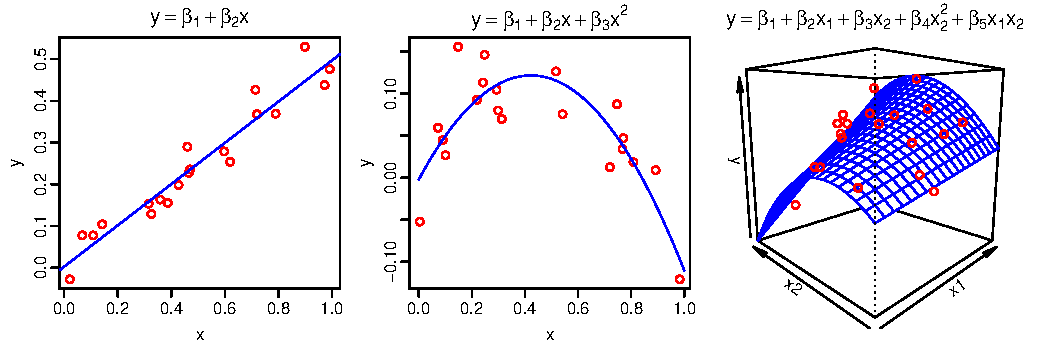
\includegraphics[width=.9\textwidth]{Linear.pdf}

	\item The data can be modelled (aka ``a mathematical model fitted to them'') as a {\it linear combination} of {\it variables} and {\it coefficients}
	\item Easily fitted using {\it Ordinary Least Squares} (OLS)
	\item Linear models can {\it include curved responses} (e.g. Polynomial regression)
\end{itemize}

% \begin{center} 
% 	{\tiny \href{https://www.mentimeter.com/s/befa8dbb37e8d1b0798e5f4669b40b67/1ba91b05de7a}{[link]}}

% 	\vspace{10pt}
% 	{\it Go to \url{www.menti.com} and enter code shown (phone or laptop)}
%   \vspace{10pt}
% \end{center}
\end{frame}


% %%%%%%%%%%%%%%%%%%%%%%%%%%%%%%%%%%%%%%%%%%%%%%%%%%%%%%
\begin{frame}{What makes a model non-linear?}

\begin{itemize}[<+->]\itemsep10pt

	\item OLS can be used to fit (model) equations that are {\it intrinsically linear},
	e.g.,
	\begin{itemize}
		\item 	Straight line: $y_i = \beta_0 + \beta_1 x_i + \varepsilon_i$
		\item Polynomial (quadratic): $y_i = \beta_0 + \beta_1 x_i + \beta_2 x_i^2 + \varepsilon_i$
		\item Another quadratic: $y_i = e^{\beta_0} + \beta_1 x_i + \beta_2 x_i^2 + \varepsilon_i$
	\end{itemize} 	
	\item What is {\it intrinsic linearity}? --- 
	the equation of the model to be fitted should be {\it linear in the parameters} (the $\beta$'s)	
	\item Some non-linear models:  
	\begin{itemize}
		\item $y_i = \beta_0 x_i^{\beta_1} + \varepsilon_i$
		\item $y_i = \beta_0 + \beta_1 x_i^{\beta_2} + \varepsilon_i$
		\item $y_i = \beta_0 e^{\beta_2 x_i} + \varepsilon_i$
		\item $y_i = \frac{\beta_0 x_i}{\beta_1 + x_i} + \varepsilon_i$
	\end{itemize}
	\pause In all of these, at least one parameter (a $\beta$) is non-linear (e.g., $x_i^{\beta_2}$, $e^{\beta_2 x_i}$, etc.) 
		
\end{itemize}

\end{frame}

%%%%%%%%%%%%%%%%%%%%%%%%%%%%%%%%%%%%%%%%%%%%%%%%%%%%%%
\begin{frame}{The Least-Squares Solution}

{\bf Recall what the Least Squares method does:}

	\begin{itemize}[<+->] \itemsep10pt

		\item Consider data on a response variable $y$, a predictor (independent) variable $x$, and $n$ observations. 
		
		\item Say we want to fit a model to these data: $
		f(x_i,\boldsymbol\beta) + \varepsilon_i $ 
		($\boldsymbol\beta = (\beta_0, \beta_1, \ldots,\beta_k)$ are 
		the model's $k+1$ parameters) 
		
		\item An example of $f(x_i,\boldsymbol\beta) + \varepsilon_i $ could be:
		$y_i = \beta_0 + \beta_1 x_i + \varepsilon_i$ (linear regression)

		\item The objective of any {\it least squares} method is to find estimates of values of the parameters ($\hat{\beta_j}$) that {\it minimize} the sum ($S$) of squared residuals ($r_i$) (AKA RSS):
		
		$$
		\text{RSS} = S = \sum\nolimits_{i=1}^n{\left[ y_i - f(x_i,\boldsymbol\beta) 
		\right]^2} = \sum\nolimits_{i=1}^n{r_i^2}
		$$
	
	\end{itemize}

\end{frame}

%%%%%%%%%%%%%%%%%%%%%%%%%%%%%%%%%%%%%%%%%%%%%%%%%%%%%%
\begin{frame}{The Least-Squares Solution}

	\begin{itemize}[<+->] \itemsep20pt

		\item The objective of any {\it least squares} method  is to find estimates of values of the parameters ($\hat{\beta_j}$) that minimize the sum ($S$) of squared residuals ($r_i$) (AKA RSS):
		
		$$
		\text{RSS} = S = \sum\nolimits_{i=1}^n{\left[ y_i - f(x_i,\boldsymbol\beta) 
		\right]^2} = \sum\nolimits_{i=1}^n{r_i^2}
		$$
		
		\item Let's picture this using a simple (OLS) example; fitting the model $y_i  = \beta_0 + \beta_1 x_i  +\varepsilon_i$...

	\end{itemize}

	
	% \begin{columns}[T]
	% \column{\textwidth}
	% 	\animategraphics[width=\textwidth, controls, buttonsize=1em, %timeline=Varying_timeline.txt % does not work - TODO
	% 	]{10}{Varying}{}{}
	% \end{columns}
	
	\end{frame}

	{
	\setbeamercolor{background canvas}{bg=}
	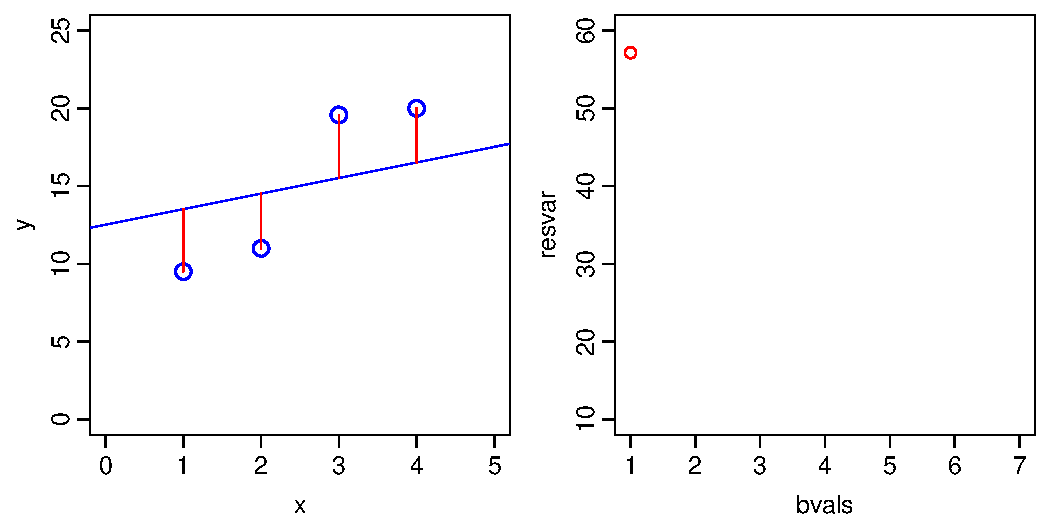
\includepdf[pages=1-50]{Varying.pdf}
	}	
%%%%%%%%%%%%%%%%%%%%%%%%%%%%%%%%%%%%%%%%%%%%%%%%%%%%%%
\begin{frame}{If the model is linear, the Least-Square solution is exact}
	
\begin{columns}[T]

	\column{0.5\textwidth}
		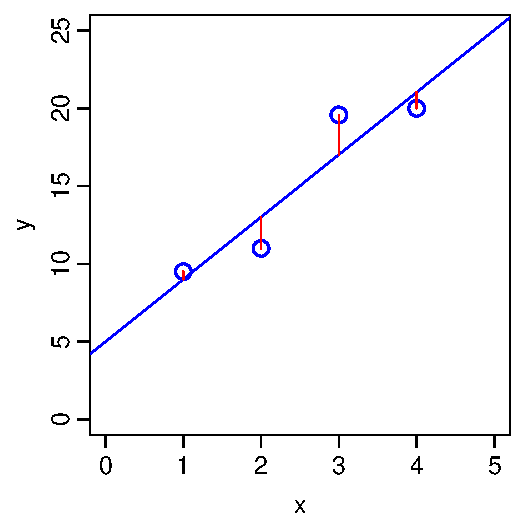
\includegraphics[width=\textwidth]{JustRight.pdf}
		
	\column{0.5\textwidth}
		\begin{align*}
		  y_i  & = \beta_0 + \beta_1 x_i  + {\color{red} \varepsilon_i }\\
		  \\
		  9.50  &= 5 + 4 \times 1 + {\color{red} 0.50}\\
		  11.00 &= 5 + 4 \times 2 - {\color{red} 2.00}\\
		  19.58 &= 5 + 4 \times 3 + {\color{red} 2.58}\\
		  20.00 &= 5 + 4 \times 4 - {\color{red} 1.00} 
		\end{align*}
		The least squares solution here is: $\beta_0 = 5; \beta_1 = 4$
				
\end{columns}		
\pause 
\begin{itemize}
	\item  \it This system of (linear) equations can be compactly represented (and solved using matrix algebra) as $\mathbf{Y} = \mathbf{X 
\boldsymbol\beta  +  \boldsymbol\varepsilon}$ 
\end{itemize}

\end{frame}

%%%%%%%%%%%%%%%%%%%%%%%%%%%%%%%%%%%%%%%%%%%%%%%%%%%%%%
\begin{frame}{Intrinsic non-linearity makes Least-Aquares model fitting difficult}

\begin{itemize}[<+->]\itemsep10pt

	\item In an {intrinsically non-linear model} such as $y_i = \beta_0
	e^{\beta_2 x_i} + \varepsilon_i$, the nice trick of solving  $\mathbf{Y} =
	\mathbf{X \boldsymbol\beta  + \boldsymbol\varepsilon}$ {\it exactly} is
	impossible	

\end{itemize}

\pause 
\begin{center}
	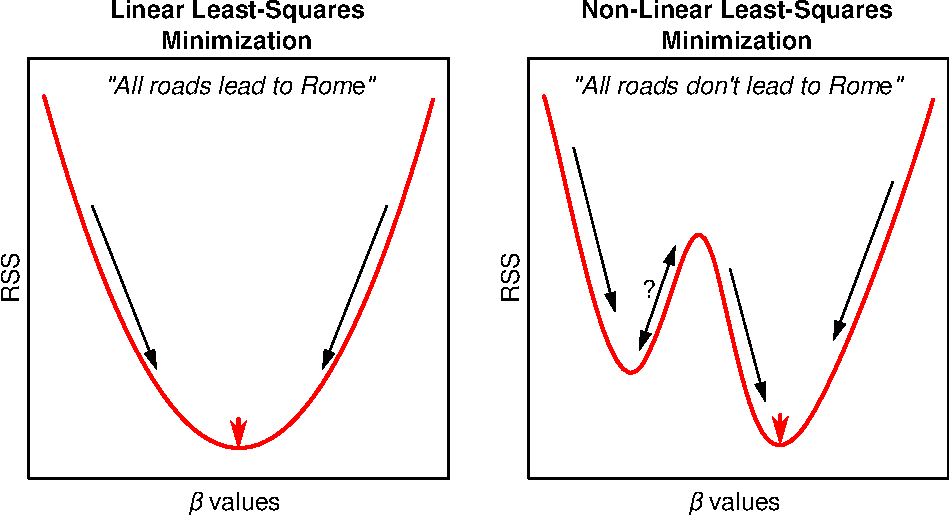
\includegraphics[width=.9\textwidth]{graphics/RSS_min.pdf}
\end{center}

\end{frame}

%%%%%%%%%%%%%%%%%%%%%%%%%%%%%%%%%%%%%%%%%%%%%%%%%%%%%%
\begin{frame}{OK, fine, why would {\it I} ever need NLLS?}

	\begin{itemize}[<+->]\itemsep10pt
		\pause 
		\item Many observations in biology are just {\it not} well-fitted by a linear model
	
		\item That is, the underlying biological phenomena/phenomenon are not 
		well-described by a linear equation
		
		\item Examples:
	
		\begin{itemize}\itemsep2pt
		
			\item Michaelis-Menten biochemical (reaction) kinetics
			
			\item Allometric growth
		
			\item Responses of metabolic rates to changing temperature 
	
			\item Consumer-Resource (e.g., predator-prey) functional responses 
			
			\item Individual growth
	
			\item Population growth
	
			\item Time-series data (e.g., fitting a sinusoidal function)
				
		\end{itemize}
	
		\item \it Can you think of some examples? 
	
	\end{itemize}
	
\end{frame}
	
%%%%%%%%%%%%%%%%%%%%%%%%%%%%%%%%%%%%%%%%%%%%%%%%%%%%%
\begin{frame}{Non-Linear Model Example: Temperature and metabolism}
		  
	\begin{columns}[c]
	  \column{2.1in}
	    \pause
	      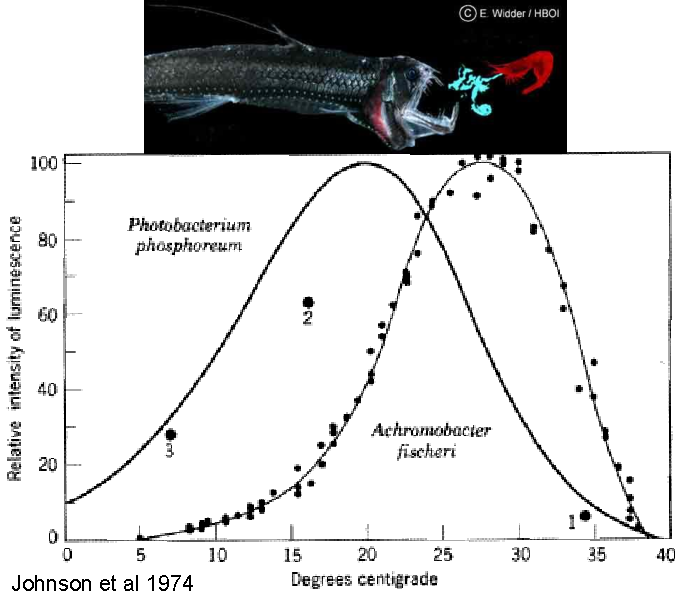
\includegraphics[width=\textwidth]{graphics/Photobacterium.pdf}
	  \pause
	  \column{2.7in}
	    $B = B_0 \boxed {e^{-\frac{E}{kT}}}f(T,T_{pk},E_D)$\\
	    \vspace{10pt}
	    \raggedright{$T$ = temperature (K)\\
	     $k$ = Boltzmann constant (eV K$^{-1}$)}\\
	     $E$ = Activation energy (eV)\\
	     $T_{pk}$ = Temperature of peak performance\\
	     $E_D$ = Deactivation energy (eV)\\
	    {\small (J H van’t Hoff 1884, S Arrhenius 1889)}
	\end{columns}
	 
\end{frame}
	
	%%%%%%%%%%%%%%%%%%%%%%%%%%%%%%%%%%%%%%%%%%%%%%%%%%%%%%
	% \begin{frame}{Example: Functional responses}
	 
	% \begin{columns}[c]
	%   \column{2in}
	%   \begin{center}
	% 			   $f(x_R) = \frac{{a x_R^{q + 1}}}{{1 + h a x_R^{q + 1}}}$
	% 	\scriptsize (Holling, 1959)
	% 	\end{center}
	%  \scriptsize
	%  $x_R$ = Resource density (Mass / Area or Volume)\\
	%  $a$ = Search rate (Area or Volume / Time )\\
	%  $h$ = Handling time \\
	%  $q$ = Shape parameter (dimensionless) 
	%  \column{2.3in}
	%       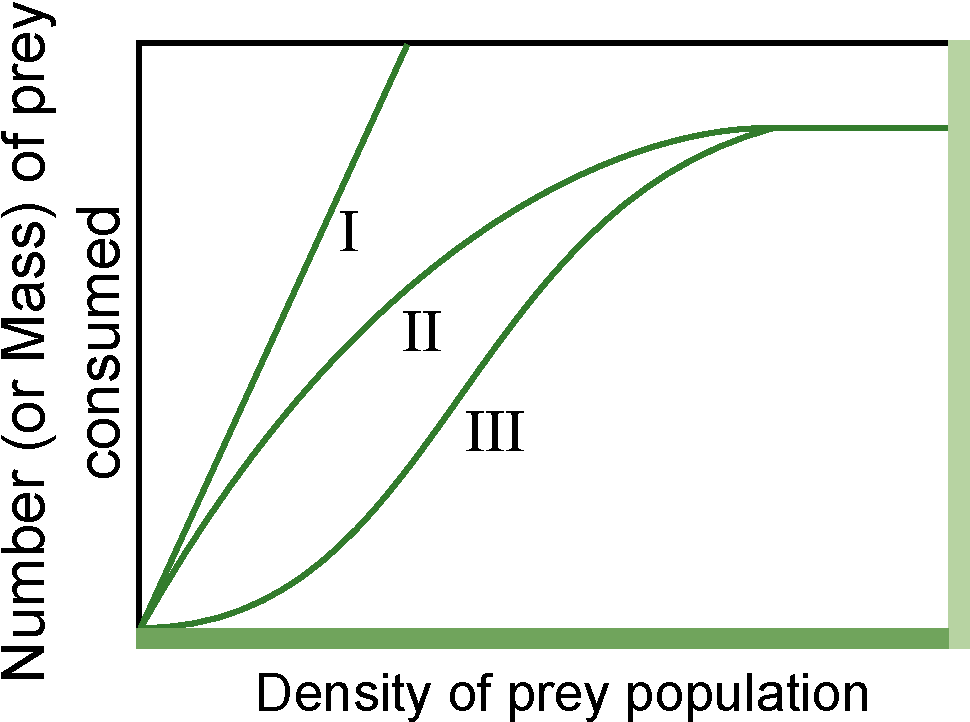
\includegraphics[width=\textwidth]{graphics/FR.pdf}
	% \end{columns}
	
	% \vspace{10pt}
	%  Note that: 
	% \begin{itemize}
	% \item NLLS fitting can yield $h < 0$, $q < 0$, or both 
	% \item $h < 0$ is biologically impossible but indicates an upward curving response
	% \item $q < 0$ is biologically unlikely as it indicates a decline in 
	% search rate with resource density (but is useful as a measure of 
	% deviation away from a type III response) 
	% \end{itemize}
	
	% \end{frame}
	
%%%%%%%%%%%%%%%%%%%%%%%%%%%%%%%%%%%%%%%%%%%%%%%%%%%%%%
\begin{frame}[plain]
 
	\begin{center}\LARGE 
		\textsc{The NLLS Fitting Method}
	\end{center}

\end{frame}

%%%%%%%%%%%%%%%%%%%%%%%%%%%%%%%%%%%%%%%%%%%%%%%%%%%%%%
\begin{frame}{The NLLS method: Overview}

	\begin{itemize}[<+->]\itemsep10pt
			
		\item OK, so we cannot find an exact, simple solution to the least-squares problem for non-linear models    
		
		\item But we can use a computer to find a {\it approximate but close-to-optimal} least-squares solution as follows:
		
		\begin{itemize}[<+->]\itemsep6pt
			\item Choose starting (initial values for the parameters we want to estimate ( $\beta_j$'s)
		
			\item Then, adjust the parameters {\it iteratively} (using a specific ``algorithm'' that is better than searching {\it randomly}) such that the RSS is gradually decreased 
	
			\item Eventually, if it all goes well, a combination of
		$\beta_j$'s that is {\it very close} to the desired solution (where the RSS is {\it approximately} minimized) can be found
				
		\end{itemize}
	\end{itemize}
	
	\end{frame}
	
%%%%%%%%%%%%%%%%%%%%%%%%%%%%%%%%%%%%%%%%%%%%%%%%%%%%%%
\begin{frame}{The NLLS fitting / optimization process}

	\begin{center}
		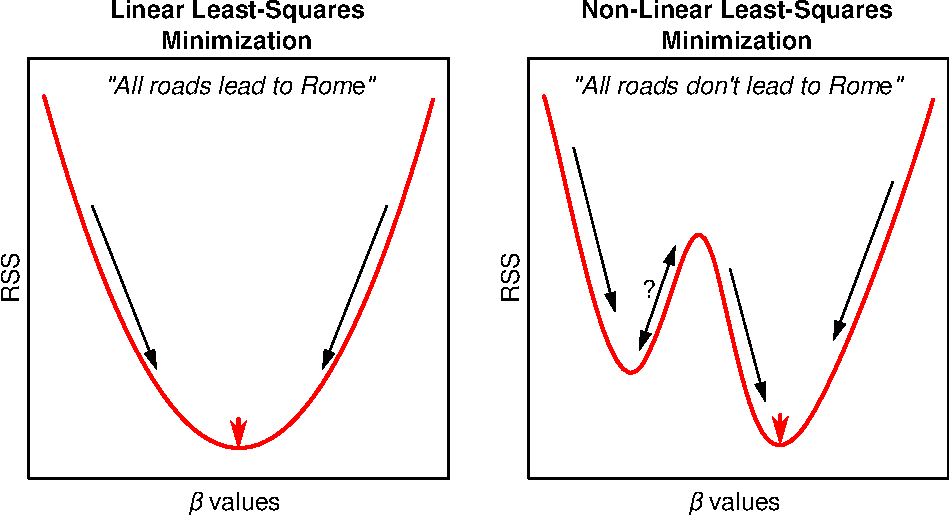
\includegraphics[width=\textwidth]{graphics/RSS_min.pdf}
	\end{center}

\end{frame}


%%%%%%%%%%%%%%%%%%%%%%%%%%%%%%%%%%%%%%%%%%%%%%%%%%%%%%

\begin{frame}{The NLLS fitting / optimization process}

The general procedure / algorithm is:

\begin{enumerate}[<+->] \itemsep4pt
	\item Start with an initial value for each parameter in the model
	\item Generate the curve defined by the initial values
	\item Calculate the residual sum-of-squares (RSS)
	\item Adjust the parameters to make the curve come closer to the data 
	points. {\it This the tricky part --- more on this in the next slide}
	\item Adjust the parameters again so that the curve comes even closer 
	to the points (RSS decreases)
	\item Repeat 4--5
	\item Stop simulations when the adjustments make virtually no 
	difference to the RSS
\end{enumerate}


\end{frame}

%%%%%%%%%%%%%%%%%%%%%%%%%%%%%%%%%%%%%%%%%%%%%%%%%%%%%%

\begin{frame}{NLLS fitting / optimization algorithms}

The {\it tricky part --- adjust parameters to make curve come closer to 
the data points} (step 4) --- has two main algorithms that are generally used:

\begin{itemize}[<+->]\itemsep10pt

	\item The {\bf Gauss-Newton} algorithm is often used, but doesn't work very well if the model to be fitted is mathematically complicated (the parameter search ``landscape'' is difficult) and the {\it starting values} for parameters are far-off-optimal
	
	\item The {\bf Levenberg-Marquardt} algorithm switches between
	Gauss-Newton and ``gradient descent'' and is more robust against starting
	values that are far-off-optimal and is more reliable in most scenarios.  
	
\end{itemize}   

\end{frame}

%%%%%%%%%%%%%%%%%%%%%%%%%%%%%%%%%%%%%%%%%%%%%%%%%%%%%%
\begin{frame}{NLLS fits -- assessment and reporting}

\begin{itemize}[<+->] \itemsep6pt
\item Once the NLLS fitting is done, you need to get the {\it goodness of fit measures}

\item First, of course, examine the fits visually

\item Report the goodness-fit results:

	\begin{itemize}
	
		\item Sums of deviations of the data points from the final model 
		fit (final RSS)
		\item Estimated coefficients
		\item For each coefficient, standard error (can be used for CI's), t-statistic and corresponding (two-tailed) p-value 
	\end{itemize} 

\item You will learn to calculate all these in the practicals   

\item You may also want to {\it compare and select between multiple competing  models}  

\item Unlike Linear Models, R$^2$ values {\it should not} be used to interpret the quality of the fit of NLLS fit (more on this in the practicals).    

\end{itemize}

\end{frame}

%%%%%%%%%%%%%%%%%%%%%%%%%%%%%%%%%%%%%%%%%%%%%%%%%%%%%%
\begin{frame}{NLLS Assumptions}

NLLS-regression has all the assumptions of OLS-regression:
	\begin{itemize}[<+->]\itemsep10pt
		
		\item No (in practice, minimal) measurement error in explanatory 
		variable ($x$-axis variable)
		
		\item Data have constant normal variance --- errors in the $y$-axis 
		are homogeneously distributed over the $x$-axis range
		
		\item The measurement/observation errors are Normally distributed (Gaussian) 
		% \pause 
		% --- for example, what would the error distribution of this 
		% non-linear model be: $y_i = \beta_0 e^{\beta_2 x_i} + 
		% \varepsilon_i$? \pause
		
		\item What if the errors are not normal? --- Interpret results
		cautiously, and use Maximum Likelihood or Bayesian fitting methods instead
	
	\end{itemize}
\end{frame}

%%%%%%%%%%%%%%%%%%%%%%%%%%%%%%%%%%%%%%%%%%%%%%%%%%%%%%
\begin{frame}[plain]
 
	\begin{center}\LARGE 
		\textsc{Practicals Overview}
	\end{center}

\end{frame}


%%%%%%%%%%%%%%%%%%%%%%%%%%%%%%%%%%%%%%%%%%%%%%%%%%%%%%

\begin{frame}{NLLS Fitting Practicals}
	
	\begin{itemize}[<+->]\itemsep16pt
	
		\item We will use {\tt R}
		
		\item For fitting simple non-linear models, the {\tt nls} function in R is sufficient 
			\begin{itemize}
				\item It uses the {\bf Gauss-Newton} algorithm by default
				\item The command is {\tt nls()}
				\item It is part of the {\tt stats} base package (so no extra installation and loading of package necessary)
			\end{itemize} 
			 
		\item For fitting complex non-linear models the {\bf Levenberg-Marquardt
		(LM)} algorithm is better

		\begin{itemize}
			\item The command is {\tt nlsLM()}
			\item It is available through the the {\tt minpack.lm} package {\small \url{http://cran.r-project.org/web/packages/minpack.lm}}
			\item It offers additional features like the ability to ``bound'' parameters to realistic values
		\end{itemize} 

	\end{itemize}   
	
	\end{frame}
	
%%%%%%%%%%%%%%%%%%%%%%%%%%%%%%%%%%%%%%%%%%%%%%%%%%%%%
\begin{frame}{NLLS Fitting Practicals}

\begin{itemize}\itemsep10pt

	\item We will start with NLLS fitting of the Michaelis-Menten model of biochemical reaction kinetics:

\end{itemize}
	
\begin{columns}[c]
	\column{.6\textwidth}
	\begin{center}
	$V = \frac{V_{\max}[S]}{K_{m} + [S]}$
	\end{center}

\begin{itemize} \scriptsize
	\item $S$ = Substrate density
	
		\item $V_{\max}$ = Maximum reaction rate (at saturating substrate concentration)
	
	\item $K_M$ = Half-saturation constant; the $S$ at which reaction rate reaches half of possible maximum ($=\frac{1}{2}V_{\max}$)
\end{itemize}
	
\column{.4\textwidth}
		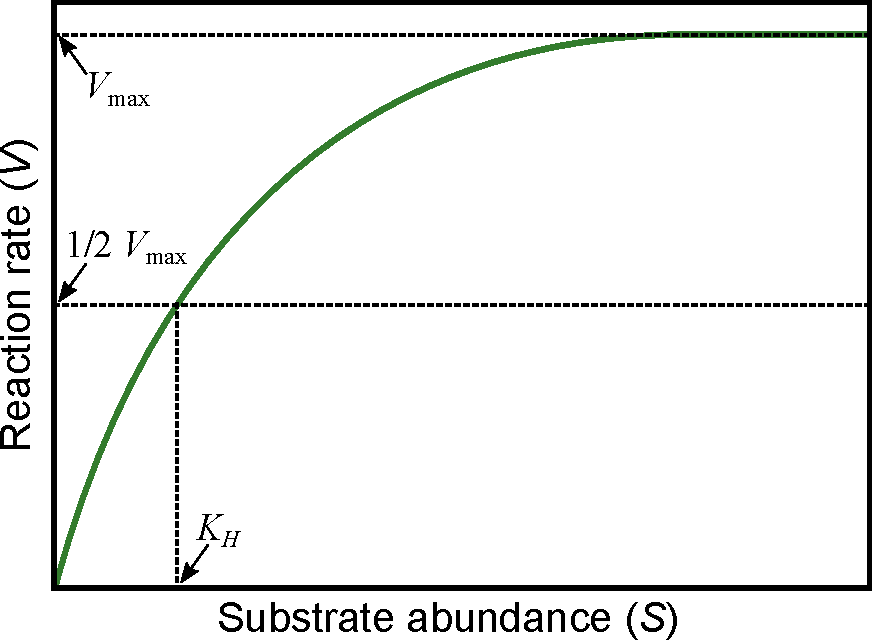
\includegraphics[width=\textwidth]{graphics/MM.pdf}
\end{columns}

\vspace{10pt}
\begin{itemize}\itemsep10pt

	\item You will use NLLS fitting to obtain estimates of $V_{\max}$ and $K_M$

	\item Note that $V_{\max} \le 0 $ and $K_M \le 0$ are physically impossible (useful fir picking starting values)

\end{itemize}

\end{frame}
	
%%%%%%%%%%%%%%%%%%%%%%%%%%%%%%%%%%%%%%%%%%%%%%%%%%%%%%

% \begin{frame}{More NLLS tips}

% \begin{itemize}[<+->]\itemsep10pt
% 	\item You can use mixed-effects modelling with NLLS in R; the package is {\tt nlme}
% 	{\small \url 
% 	{https://stat.ethz.ch/R-manual/R-devel/library/nlme/html/nlme.html}}
% 	(You are probably stuck with the Gauss-Newton algorithm with 
% 	{\tt nlme} though)
	
% 	\item You can also use Python --- look up {\tt lmfit} \url{https://lmfit.github.io/lmfit-py/index.html}. \\ {\tt python} seems to have a better Levenberg-Marqualdt implementation than {\tt R} 
	
% \end{itemize}   

% \end{frame}

%%%%%%%%%%%%%%%%%%%%%%%%%%%%%%%%%%%%%%%%%%%%%%%%%%%%%%

\begin{frame}{Readings}

\begin{itemize}\itemsep16pt
	
	\item Motulsky, Harvey, and Arthur Christopoulos. Fitting models to 	biological data using linear and nonlinear regression: a practical 
	guide to curve fitting. OUP USA, 2004. 
	
	% \item Johnson, J. B. \& Omland, K. S. 2004 Model selection in ecology and evolution. Trends Ecol. Evol. 19, 101--108. 

\end{itemize}   

\end{frame}

% %%%%%%%%%%%%%%%%%%%%%%%%%%%%%%%%%%%%%%%%%%%%%%%%%%%%%%
% \begin{frame}{Why is intrinsic non-linearity a problem?}

% % {\bf Let's use maths instead of brute-force computation!}

% 	\begin{itemize}[<+->] \itemsep16pt

% 		\item Our model is $f(x_i,\boldsymbol\beta) + \varepsilon_i$ \\ 
			
% 		\item We want to find estimates of values of the parameters 
% 		($\hat{\beta_j}$) that {\it minimize} the sum ($S$) of squared residuals 
% 		($r_i$) (AKA ``RSS'') $S = \sum\nolimits_{i=1}^n{\left[ y_i - 
% 		f(x_i,\boldsymbol\beta) \right]^2} = \sum\nolimits_{i=1}^n{r_i^2}$

% 		\item For this we can solve $\frac{\partial S}{\partial 
% 		\beta_j} = 0, j = 0,1,2,\ldots,k$ to find the {\it minimum}
	
% 		\item That is, we need to solve	
% 		$\frac{\partial \sum\nolimits_{i=1}^n{r_i^2}}{\partial \beta_j} = 
% 		0$
		
% 		\item Or, $2 \sum\nolimits_{i=1}^n r_i \frac{\partial r_i}{\partial \beta_j} = 0$
	
% 	\end{itemize}

% \end{frame}

% %%%%%%%%%%%%%%%%%%%%%%%%%%%%%%%%%%%%%%%%%%%%%%%%%%%%%%
% \begin{frame}{Why is intrinsic non-linearity a problem?}

% 	\begin{itemize}[<+->] \itemsep16pt

% 		\item Thus, solving $ 2 \sum\nolimits_{i=1}^n r_i \frac{\partial r_i}{\partial \beta_j} 
% 		= 0$ \\
		
% 		boils down to finding the ``gradient'' $ \frac{\partial r_i}{\partial \beta_j} $
	
% 		\item This is not a problem in linear models, because this gradient 
% 		is fully solvable as the equation is {\it intrinsically linear}
		
% 		\item That is, the solution of $ \frac{\partial r_i}{\partial 
% 		\beta_j} $ is simple (enough)  
				
% 	\end{itemize}

% \end{frame}

% %%%%%%%%%%%%%%%%%%%%%%%%%%%%%%%%%%%%%%%%%%%%%%%%%%%%%%
% \begin{frame}{Why is intrinsic non-linearity a problem?}

% 	\begin{itemize}[<+->] \itemsep16pt
		
% 		\item For example, if $f(x_i,\boldsymbol\beta) + \varepsilon_i = \beta_0 + \beta_1 x_i + 
% 		\varepsilon_i$ \\
		
% 		\item That is, our model is $y_i = \beta_0 + \beta_1 x_i + \varepsilon_i$ 
% 		(Linear Regression)
		
% 	\item Then we want to solve 
		
% 		$\frac{\partial S}{\partial {\beta_0}} = 
% 		\sum\nolimits_{i=1}^{n}{\frac{\partial {{\left[ 
% 		y_i-(\beta_0+\beta_1 x_i) \right]}^{2}}}{\partial {{\beta 
% 		}_{0}}}}=0 $ \\
		 
% 		$ \frac{\partial S}{\partial {{\beta 
% 		}_{1}}}=\sum\nolimits_{i=1}^{n}{\frac{\partial {{\left[ 
% 		{{y}_{i}}-({{\beta }_{0}}+{{\beta }_{1}}{{x}_{i}}) 
% 		\right]}^{2}}}{\partial {{\beta }_{1}}}} = 0$
		
% 	\end{itemize}

% \end{frame}

% %%%%%%%%%%%%%%%%%%%%%%%%%%%%%%%%%%%%%%%%%%%%%%%%%%%%%%
% \begin{frame}{Why is intrinsic non-linearity a problem?}

% 	\begin{itemize}[<+->] \itemsep16pt

% 		\item And, solving\\ 		
% 		$\frac{\partial S}{\partial {\beta_0}} = 
% 		\sum\nolimits_{i=1}^{n}{\frac{\partial {{\left[ 
% 		y_i-(\beta_0+\beta_1 x_i) \right]}^{2}}}{\partial {{\beta 
% 		}_{0}}}}=0 $\\ 
		 
% 		$ \frac{\partial S}{\partial {{\beta }_{1}}}=\sum\nolimits_{i=1}^{n}{\frac{\partial 
% 		{{\left[ {{y}_{i}}-({{\beta }_{0}}+{{\beta }_{1}}{{x}_{i}}) 
% 		\right]}^{2}}}{\partial {{\beta }_{1}}}} = 0$ \\
		
% 		\vspace{6pt}
% 		just boils down to solving two simultaneous equations because $ 
% 		\frac{\partial r_i}{\partial \beta_j} $ is simple {\it because} the model 
% 		is intrinsically linear:\\
		
% 		\vspace{6pt}
% 		$-n{{\beta }_{0}}+\sum\nolimits_{i=1}^{n}{{{y}_{i}}}+{{\beta 
% 		}_{1}}\sum\nolimits_{i=1}^{n}{{{x}_{i}}}=0 $\\ 
		
% 		$ \sum\nolimits_{i=1}^{n}{{{x}_{i}}{{y}_{i}}}-{{\beta 
% 		}_{0}}\sum\nolimits_{i=1}^{n}{{{x}_{i}}}+{{\beta 
% 		}_{1}}\sum\nolimits_{i=1}^{n}{x_{i}^{2}}=0$

% 		\item That is, we need to solve $\mathbf{Y} = \mathbf{X 
% 		\boldsymbol\beta  +  \boldsymbol\varepsilon}$ ({\it this is what R 
% 		solves when you use {\tt lm()}})

% 	\end{itemize}

% \end{frame}


%%%%%%%%%%%%%%%%%%%%%%%%%%%%%%%%%%%%%%%%%%%%%%%%%%%%%%
\end{document}
